% !TeX spellcheck = it\_IT
\documentclass{article}

\usepackage{arxiv}

\usepackage[utf8]{inputenc} % allow utf-8 input
\usepackage[T1]{fontenc}    % use 8-bit T1 fonts
\usepackage{hyperref}       % hyperlinks
\usepackage{url}            % simple URL typesetting
\usepackage{booktabs}       % professional-quality tables
\usepackage{amsfonts}       % blackboard math symbols
\usepackage{nicefrac}       % compact symbols for 1/2, etc.
\usepackage{microtype}      % microtypography
\usepackage{lipsum}		% Can be removed after putting your text content
\usepackage{listings}
\usepackage{url}
\usepackage{graphicx}
\usepackage{longtable}
\usepackage{float}

\renewcommand{\figurename}{Figura}
\renewcommand{\tablename}{Tabella}

\lstset{
	basicstyle=\ttfamily\footnotesize
}  

\title{Approfondimento}

\renewcommand{\headeright}{}

\begin{document}
	
\section{Hook ed ErrorHook}
\subsection{OSEK/VDX}
La specifica OSEK/VDX definisce le \textit{hook routines} come un mezzo per consentire azioni definite dall'utente riferite a processi interni del sistema operativo. Queste hanno alcune caratteristiche specifiche:

\begin{itemize}
\item sono chiamate dal sistema operativo, in un contesto speciale dipendente dal sistema operativo;
\item con priorità maggiore di tutti i \textit{task};
\item non possono essere interrotte da ISR2;
\item con un'interfaccia standardizzata, ma con funzionalità non standardizzate (perchè definite dall'utente).
\end{itemize}

Esse possono essere utilizzate allo \textit{startup} del sistema (\textit{StartupHook}), al suo \textit{shutdown (ShutdownHook)}, per \textit{debugging (PreTaskHook/PostTaskHook/IdleHook)} o per \textit{error handling (ErrorHook)}.

La maggior parte dei servizi del sistema operativo non è consentita per le \textit{hook routines}. Questa restrizione è necessaria per ridurre la complessità del sistema.

La \textit{routine ErrorHook} viene chiamata se un servizio del sistema operativo restituisce un valore di \textit{StatusType} diverso da 'E\_OK'. Lo scopo dell'\textit{ErrorHook} è quindi di trattare in modo centralizzato alcuni errori del sistema operativo relativi all'esecuzione del sistema.

\subsection{ERIKA³}
Nello specifico dell'attivazione di un \textit{task}, i possibili valori di \textit{StatusType} sono 'E\_OK', 'E\_OS\_LIMIT', 'E\_OS\_ID' (solo per \textit{task} di tipo \textit{extended}). Lo stato di interesse è 'E\_OS\_LIMIT', che identifica troppe attivazioni pendenti di un \textit{task}. È importante notare come questo stato sia possibile solamente per primitive di tipo \textit{ActivateTask} e \textit{ChainTask} e attivazioni del \textit{task} allo scattare di un allarme.

Un allarme (\textit{Alarm}) è un meccanismo di notifica collegato a uno specifico \textit{Counter} che, una volta raggiunto il \textit{tick} stabilito, definito nel \textit{file} OIL, può attivare un \textit{task}, impostare un evento o invocare una \textit{callback}. L'esecuzione della notifica relativa a un allarme avviene all'interno della funzione \textit{IncrementCounter} che incrementa il \textit{tick} del contatore collegato a quell'allarme. Questa funzione è atomica e al suo termine avviene il \textit{rescheduling}, se questa è chiamata a livello di \textit{task}, o, se chiamata da un ISR, il \textit{rescheduling} avviene al termine dell'ISR nidificato più esterno.

Quando si cerca di attivare un \textit{task}, sia per la notifica di un allarme o una primitiva del sistema invocata dall'utente, il \textit{kernel} di ERIKA³ effettua dei controlli sullo stato dei \textit{task} del sistema e, in particolare, sullo stato della coda dei pronti. Se il \textit{task} interessato dall'attivazione non ha \textit{job} nella coda dei pronti (quindi inevitabilmente il numero di attivazioni di quel \textit{task} è pari a 0) lo aggiunge a questa, mentre se ci sono già suoi \textit{job} in attesa (in stato \textit{'ready'} o \textit{'waiting'}) o in esecuzione (stato \textit{'running'}), viene valutato il numero di attivazioni pendenti di quel \textit{task} in quel momento e confrontato con il numero di attivazioni massime impostato nel \textit{file} OIL. Il valore di attivazioni pendenti a \textit{runtime} viene quindi modificato in due momenti:

\begin{itemize}
\item All'attivazione del \textit{task}, sia questa causata da un allarme o dalle primitive \textit{ActivateTask/ChainTask}, viene invocata la funzione 'osEE\_handle\_action', la quale a sua volta chiama 'osEE\_task\_activated'. Questa, come si può vedere dal codice riportato nella Figura \ref{act}, verifica il valore del numero di attivazioni pendenti del \textit{task} a cui fa riferimento il parametro passato nella chiamata e, se minore del numero massimo di attivazioni impostate per quel \textit{task}, aumenta il numero di attivazioni pendenti e imposta la variabile che identifica lo \textit{StatusType} a 'E\_OK', in caso contrario imposta quest'ultima a 'E\_OS\_LIMIT'.
\item Al termine dell'esecuzione del \textit{task} viene invocata la funzione 'osEE\_task\_end' che, come si può vedere nella Figura \ref{act} diminuisce il valore del numero di attivazioni pendenti del \textit{task} a cui fa riferimento il parametro passato nella chiamata e modifica lo stato del \textit{task} in base al numero di attivazioni pendenti rimanenti.
\end{itemize}

\begin{figure}[!htbp]
	\centering
	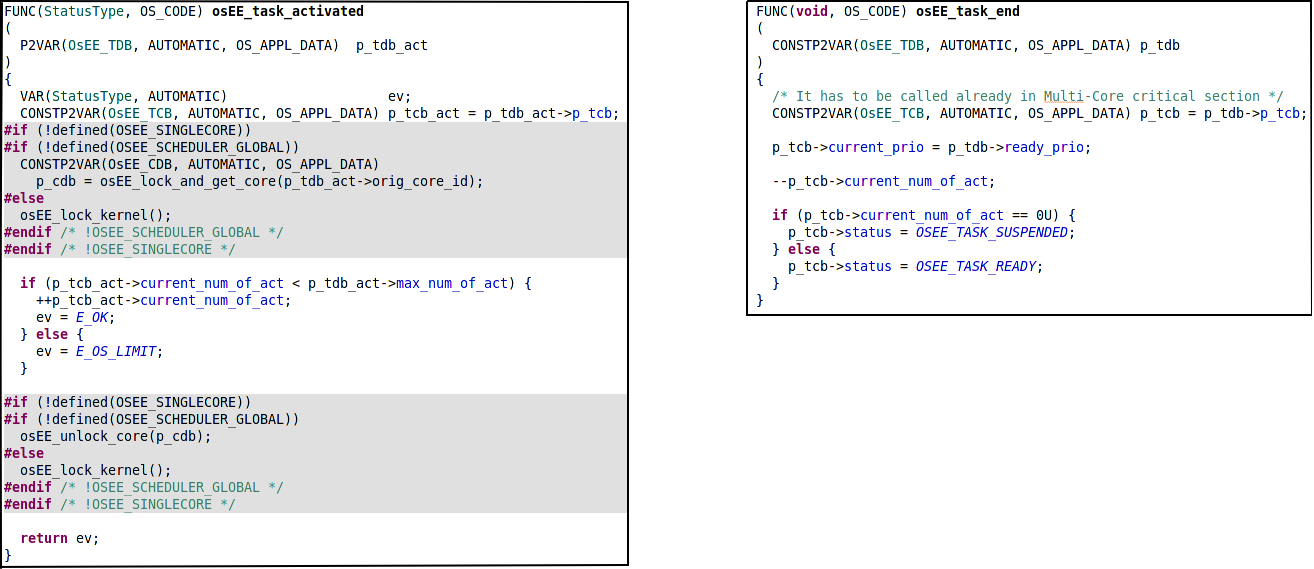
\includegraphics[width=5in]{Approfondimento/osEE_task_activated_end.png}
	\caption{Funzioni 'osEE\_task\_activated' e 'osEE\_task\_end'}
	\label{act}
\end{figure}

Durante l'attivazione del \textit{task}, se il valore di \textit{StatusType} definito dalla variabile 'ev' nel codice in Figura \ref{act} è diverso da 'E\_OK', la funzione 'osEE\_handle\_action' invoca la funzione 'osEE\_call\_error\_hook' che a sua volta chiama la funzione 'ErrorHook' implementata dall'utente come definito nello standard OSEK/VDX.

In Figura \ref{stack} è riportato lo \textit{stack} delle chiamate nel caso di invocazione dell'\textit{ErrorHook}.

\begin{figure}[!htbp]
	\centering
	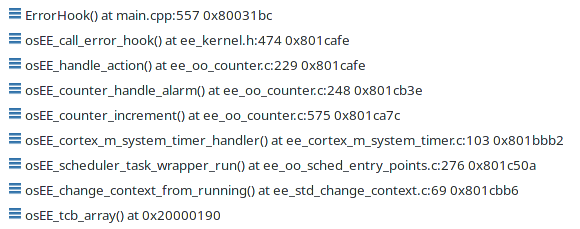
\includegraphics[width=3in]{Approfondimento/Stack_ErrorHook.png}
	\caption{\textit{Stack} delle chiamate a \textit{ErrorHook}}
	\label{stack}
\end{figure}

\subsection{UTILIZZO COME METRICA PER \textit{DEADLINE-MISS}}
Utilizzare il numero di errori di attivazione sfruttando \textit{ErrorHook} ha certamente delle limitazioni in base alla configurazione del sistema, ed è utilizzabile solamente nel caso di \textit{task} con \textit{deadline} implicita in cui, se non si hanno \textit{deadline miss}, l'attivazione di un \textit{task} avviene quando questo non ha attivazioni pendenti. Nel mio progetto i \textit{task} di interesse sono periodici e con \textit{deadline} implicite, quindi utilizzare questo metodo come metrica per contare le \textit{deadline miss} mi è sembrato di semplice attuazione e sufficiente per lo scopo.

P.S.: dopo aver effettuato l'approfondimento sottostante, ho realizzato che questo metodo soffre di una mancanza molto importante, che gli permette di identificare solamente alcune \textit{deadline miss}. Ricordando che nell'esempio di prova i \textit{task} possono avere al più un solo \textit{job} nella coda dei pronti contemporaneamente, quando arriva una nuova richiesta di attivazione di un \textit{task}, il sistema può essere in diverse situazioni:
\begin{itemize}
	\item il \textit{task} in questione non ha alcun \textit{job} nella coda dei pronti, e dunque dopo l'attivazione un nuovo \textit{job} viene inserito in questa nello stato \textit{'ready'};
	\item il \textit{task} in questione ha un \textit{job} nella coda dei pronti, sia questo in esecuzione o no: in questo caso il meccanismo che utilizza \textit{ErrorHook} identifica la \textit{deadline miss}, ma l'attivazione del nuovo \textit{job} viene persa. In questo caso, quindi, quel \textit{task} una volta terminato rimarrà in attesa di un nuovo allarme senza eseguire.
\end{itemize}
Quest'ultimo caso comporta un minor numero di attivazioni del \textit{task}, e quindi anche meno \textit{deadline miss} identificate. Questo comportamento era stato notato anche nella relazione in riferimento alla differenza di utilizzo \% della CPU con vari carichi, ma non avevo pensato a questa importante implicazione.

Stimare le \textit{deadline miss} effettive è piuttosto complesso e dipende dalle caratteristiche del sistema (priorità e tempo d'esecuzione dei \textit{task}). È possibile però definire un \textit{lower bound} al rapporto fra \textit{deadline miss} rilevate e \textit{deadline miss} effettive. Per la valutazione di questo ho mantenuto costante il tempo d'esecuzione dei \textit{player}1 e 2, modificando quindi solamente il tempo d'esecuzione del \textit{player}3.

Il caso peggiore si manifesta con la configurazione con priorità P3>P2>P1 (o P3>P1>P2), con \textit{offset} di 1ms e tempo d'esecuzione del \textit{player}3 maggiore di 10ms ma inferiore a 18ms. In questo caso le \textit{deadline miss} rilevate riguardano tutte il \textit{player}3 e sono circa 1/6 di quelle effettive, che invece interessano anche i \textit{player}1 e 2, essendo questi a priorità inferiore e il \textit{player}3 sempre in esecuzione (e avendo un \textit{utilization}>1 non terminerà mai entro la sua \textit{deadline}). Per tempi d'esecuzione del \textit{player}3 maggiori, il numero di \textit{deadline miss} rilevate è sempre inferiore a 1/3 di quelle effettive, in quanto non vengono mai considerate le \textit{deadline miss} sui \textit{player}1 e 2, ma limitate comunque rispetto al caso precedente.

In alcuni casi le \textit{deadline miss} rilevate sono invece uguali a quelle effettive: ne è un esempio l'esecuzione con priorità P3>P2>P1,  tempo d'esecuzione del \textit{player}3 pari a 9,5ms e senza alcun \textit{offset} (ma anche con \textit{offset} di 1ms la differenza è minima e si differenzia solamente per la prima esecuzione del \textit{player}1). In questo caso il \textit{task} che subisce interferenza e ha \textit{deadline miss} è il \textit{player}1, che non eseguirà mai e quindi non consumerà mai il \textit{release event} iniziale, e quindi tutte le \textit{deadline miss} sono rilevate.

Il caso peggiore con priorità P1>P2>P3 (o P2>P1>P3) si rileva con tempo d'esecuzione del \textit{player}3 maggiore di 9ms ma inferiore a 18ms, in cui le \textit{deadline miss} rilevate sono la metà delle \textit{deadline miss} effettive, in quanto il \textit{player}3 ha \textit{deadline miss} ad ogni esecuzione, ma \textit{release event} considerati esattamente la metà di quelli effettivi.

La varianza del rapporto tra \textit{deadline miss} rilevate e \textit{deadline miss} effettive è quindi elevata e stabilire un valore medio risulta complicato, soprattuto tenendo in considerazione che i \textit{test} sono stati effettuati con un valore di carico sul \textit{player}3 variabile nel tempo.

\section{Offset}

Il \textit{critical instant} di un \textit{task} $T_i$ è l'evento di rilascio di un suo \textit{job} $j_i$ al quale corrisponde la massima estensione di interferenza, da cui consegue che, il \textit{job} $j_i$ rilasciato in quell'istante, ha il valore maggiore di response time fra tutti i \textit{job} del \textit{task} $T_i$.

Nel caso di \textit{task} indipendenti fra loro, quindi senza risorse in comune o vincoli di precedenza, questo può avvenire se il \textit{job} viene rilasciato nello stesso istante di tutti i \textit{job} con priorità maggiore, e quindi deve aspettare prima di poter eseguire.

Rispetto al valore di \textit{critical instant}, quanto più vicino a questo istante viene rilasciato $j_i$, più grande sarà il suo \textit{response time}, con un limite superiore all'ampiezza di questo quando la fase di tutti i \textit{job} è pari a 0 (\textit{critical instant} al tempo 0).
Da questo consegue che con \textit{offset} pari a 0 per tutti i \textit{task} si presenta lo scenario peggiore per lo \textit{scheduling} del sistema [Liu, Layland: 1973].

Quando i \textit{task} hanno priorità fissate \textit{offline} (come nel caso di FPS), una situazione di \textit{overloading} del sistema causata da un \textit{job} di un \textit{task} non può influenzare gli altri \textit{task} a priorità maggiore. Allo stesso modo, però, una situazione di \textit{overloading} costante del sistema può causare un blocco totale dei \textit{task} a priorità inferiore del \textit{task} bloccante [Mark K. Gardner, Jane W.S. Liu: \textit{"Performance of Algorithms for Scheduling Real-Time Systems with Overrun and Overload"}].

Nei risultati ottenuti dai \textit{test} con carico riportati nella relazione, si vede infatti come la differenza fra utilizzo o meno dell'\textit{offset}, nel caso di priorità dei \textit{task player} rispettivamente P1>P2>P3 (e con prerilascio), sia pressochè inesistente. Questo a prova del fatto che i \textit{task} a priorità maggiore non subiscono interferenze dai \textit{job} in \textit{overrun} che hanno priorità minore.

Quando i \textit{task} però hanno priorità rispettivamente P3>P2>P1, e quindi il \textit{task} i cui \textit{job} causano l'\textit{overload} del sistema ha priorità maggiore degli altri \textit{task}, l'\textit{offset} diventa essenziale per ridurre il numero di \textit{deadline miss}, evitando che ci siano attivazioni dei \textit{task} nello stesso istante.

Nel mio esempio di prova, il sistema risulta in uno stato di \textit{overload} con \textit{execution time} dei \textit{job} del \textit{player}3 compreso fra 9 e 10ms.
Per quanto riguarda i \textit{job} di \textit{player}1 e \textit{player}2, è ragionevole pensare che l'\textit{execution time} di questi sia < <1ms, in quanto osservando il \textit{log} del sistema a \textit{runtime}, questi hanno sempre esecuzione <1ms e hanno lo stesso \textit{timestamp}. Non avendo un valore preciso sul tempo di esecuzione di questi, considero in questo caso un \textit{execution time} di 0,5ms.

Definiti questi tempi d'esecuzione e il periodo dei \textit{task} di 10ms, i \textit{task} rappresentanti i \textit{player}1 e 2 hanno ampi margini per completare l'esecuzione, avendo un \textit{utilization} di 0,05 ciascuno, mentre il \textit{player}3, nell'intorno del punto di rottura, di 0,95. Risulta quindi di particolare importanza applicare un \textit{offset} su quest'ultimo per ridurre le interferenze sui \textit{player}1 e 2 quando questo sia possibile. Con il \textit{player}3 che impiega 9,5ms per completare infatti, solamente il \textit{player}2 avrà il tempo di eseguire prima della \textit{deadline}, mentre il \textit{player}1 non ci riuscirà mai. In questo caso l'intero sistema ha una \textit{total utilization} > 1, che, con un'unica CPU disponibile come la \textit{board} di prova, comporta l'impossibilità ad ottenere uno \textit{schedule feasible}.

Se il carico, e dunque il tempo d'esecuzione del \textit{player3}, aumenta oltre il suo periodo, in riferimento alla configurazione del sistema di \textit{test}, la nuova attivazione viene persa.
Un esempio ti tale scenario è rappresentato da un carico sul \textit{player}3 che ne aumenta il tempo d'esecuzione a 10,5ms.
In Figura \ref{timeline} ho riportato il confronto fra l'esecuzione del sistema (considerando solamente i \textit{task player}) senza \textit{offset}, in cui si nota come si alternino le \textit{deadline miss} del \textit{player}3 e dei \textit{player}1 e 2, e del sistema con \textit{offset} uguale a 1ms, in cui le \textit{deadline miss} interessano il \textit{player3}. Per la \textit{timeline} ho considerato un tempo d'esecuzione di 2 volte l'iperperiodo + il valore dell'\textit{offset} [Leung, Merrill: "A note on preemptive scheduling of periodic, real-time tasks"].
Ho considerato un \textit{execution time} per i \textit{player}1 e 2 pari a 0,5ms, mentre per il \textit{player}3 di 10,5ms.

\begin{figure}[!htbp]
	\centering
	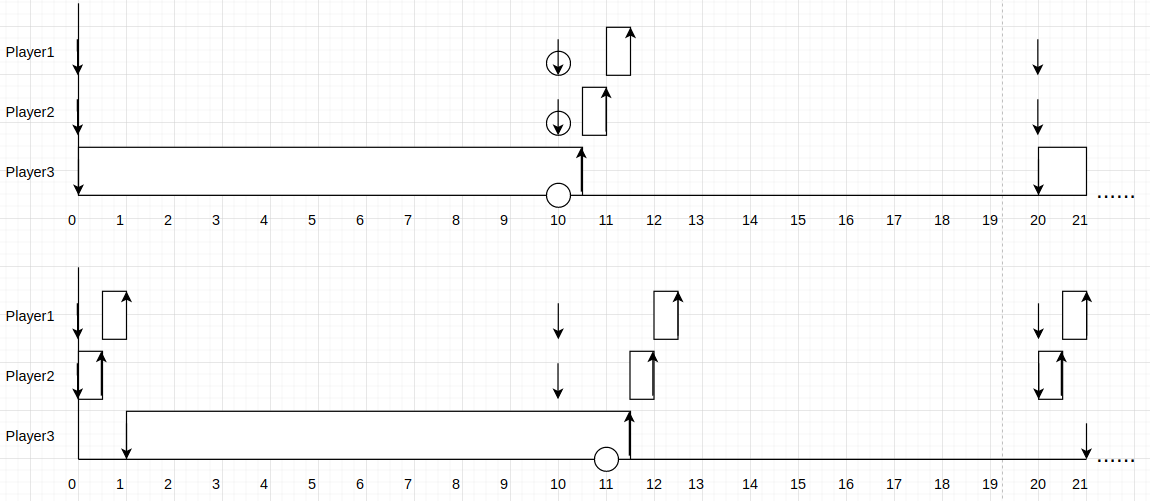
\includegraphics[width=6in]{Approfondimento/timeline.png}
	\caption{Confronto esecuzione senza e con \textit{offset}}
	\label{timeline}
\end{figure}

L'\textit{offset} si rivela dunque estremamente utile in questi casi per ridurre eventuali interferenze causate da \textit{task} a priorità maggiore, ma comporta una difficoltà maggiore nell'assegnazione di priorità ottimali ai \textit{task} [Ken Tindell: \textit{"Adding Time-Offsets to Schedulability Analysis"}].
A tal proposito, si può pensare al sistema presentato prima in cui il \textit{player}3 ha un tempo di esecuzione di 9,5ms. In questo caso, se non si applica \textit{offset}, il \textit{player}1 non eseguirà mai, ma i \textit{player}2 e 3 invece termineranno entro la loro \textit{deadline} e l'utilizzo teorico della CPU sarà del 100\%, mentre se si applica un \textit{offset} pari a 1ms i \textit{player}1 e 2 termineranno sempre, ma il \textit{player}3 avrà una \textit{deadline miss} ad ogni esecuzione, con conseguente perdita della nuova attivazione nel sistema di \textit{test} proposto.


\end{document}